%checked by mark May 9th 2019
\pagebreak
\section{Placement of Social Contacts}
\label{sec:contacts:placing}

This section looks into options of where to place social contacts relative to the user \cite{Nassani2017a} by testing two options (Figure \ref{fig:continuum:conditions}): 1) Life-sized, where social contacts are presented as human-size virtual avatars displayed around the viewer, and 2) Miniature, where the social contacts are displayed on a table-top nearby the viewer. 

\begin{figure}[ht]
    \centering
    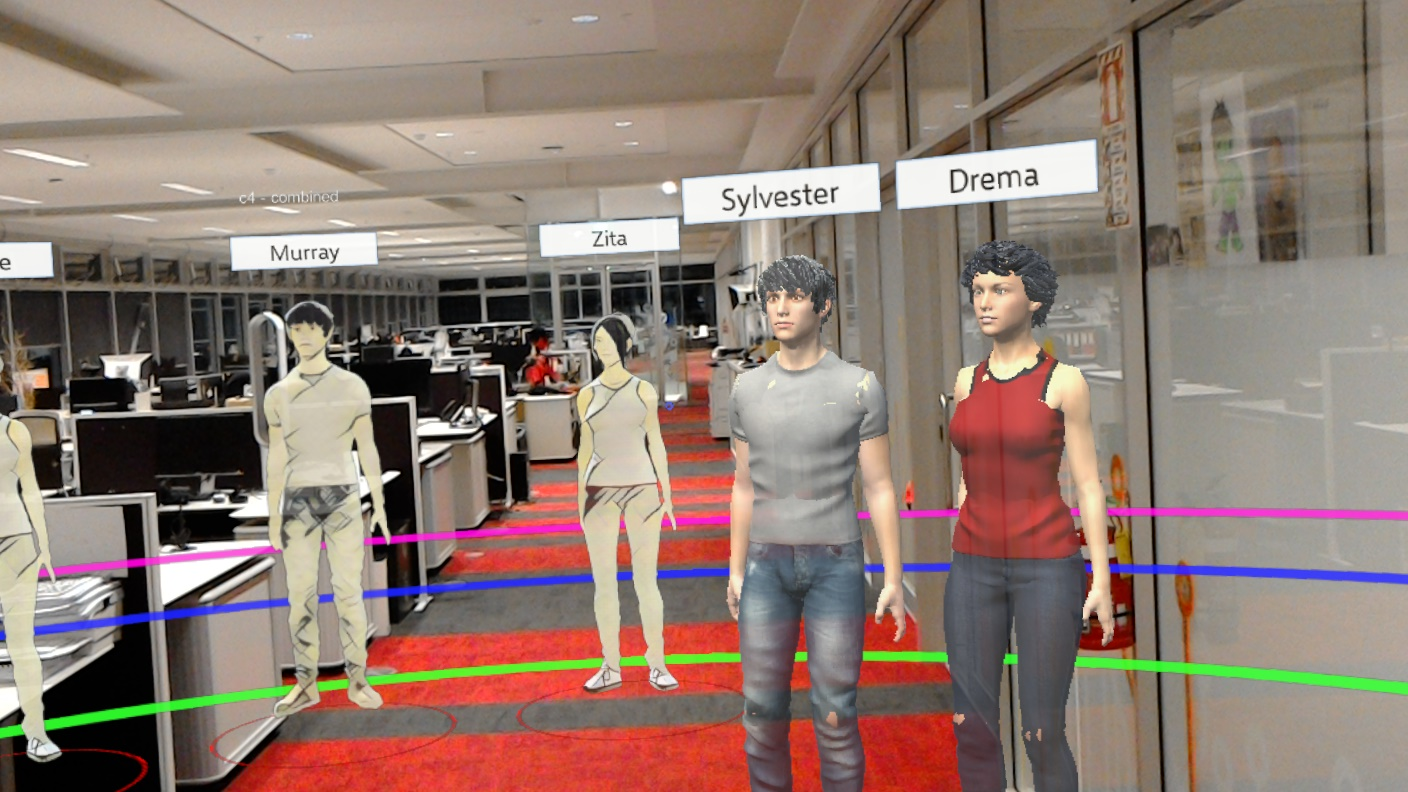
\includegraphics[width=0.8\linewidth]{images/42-placement-ismar17/20170625_205203_HoloLens.jpg}    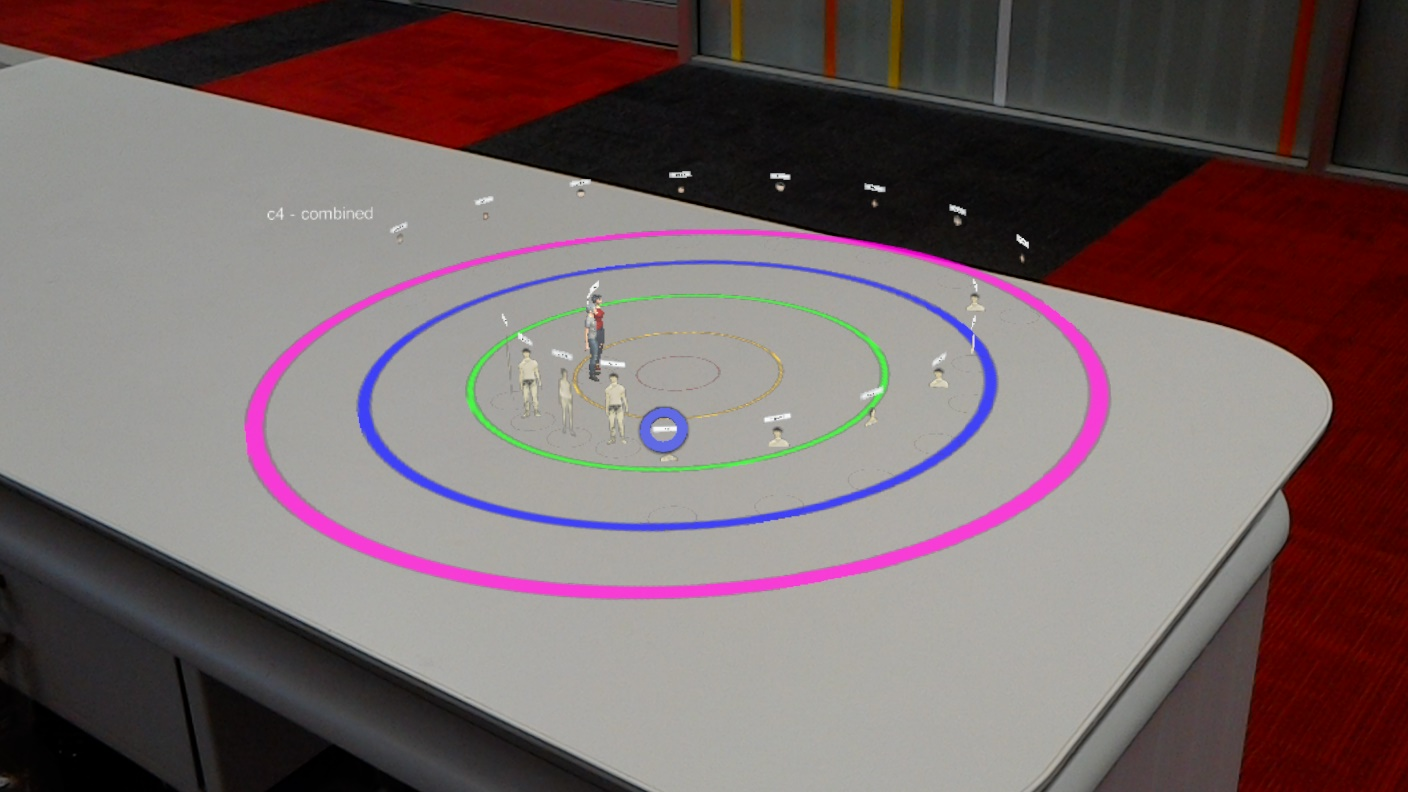
\includegraphics[width=0.8\linewidth]{images/42-placement-ismar17/20170625_205112_HoloLens.jpg}
    \caption{Prototype interfaces for contact placement. Life-sized (top) on the ground vs. Miniature (bottom) on a nearby surface.} 
    \label{fig:continuum:conditions}
\end{figure}

\subsection{Implementation}

A prototype was implemented (Figure \ref{fig:placement:system}) on the Microsoft HoloLens to test the two conditions on the contact placement dimension, one viewing avatars. The prototype also allowed the user (as a viewer) to select and move an avatar closer to or further away from the viewer position by using air-tap gestures of the HoloLens. The air-tap gesture\footnote{https://docs.microsoft.com/en-us/windows/mixed-reality/gestures} is recognised by touching the index and thumb fingers to select. The purpose of the selection and movement process was to change the social relationship between the viewer and their social contacts. When the viewer focuses on a social contact and uses the air-tap gesture, then the social contact will be able to moved from the current social proximity ciricle (e.g., Friend) to the next one (e.g. Intimate). 

\begin{figure}[ht]
    \centering
    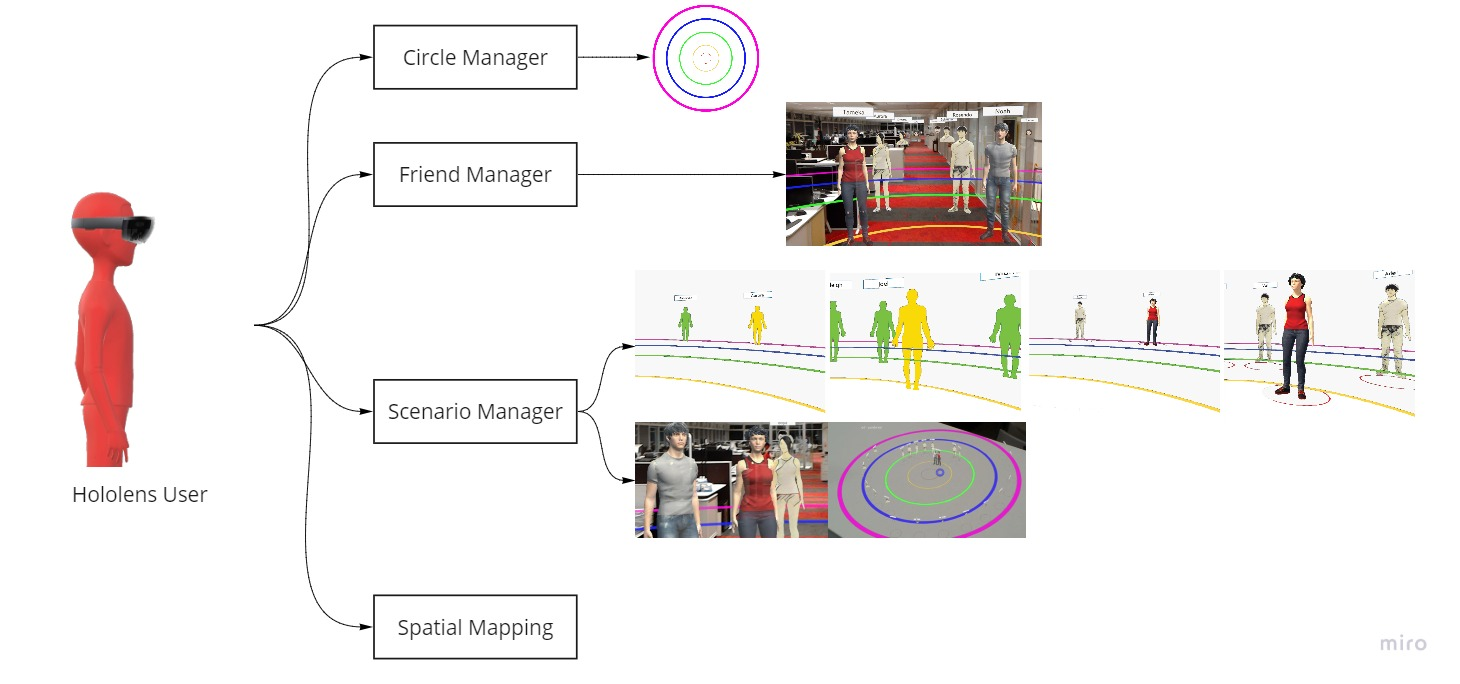
\includegraphics[width=\linewidth]{images/42-placement-ismar17/placement-system.jpg}   
    \caption{System implementation of social contacts placement on a HoloLens device} 
    \label{fig:placement:system}
\end{figure}


\subsection{User Study}

Feedback was collected from potential users during an open day at our lab as the participants tried demonstrations of the two conditions: C1-Life-sized (L) and C2-Miniature (M) representations of avatars. Twenty-seven participants tried the system prototype. On trying a demonstration of each condition, participants were asked to rate their experience on a 7-point Likert scale (where 1=not very and 7=very) for three subjective questions on: 

\begin{itemize}
    \item Q1: How easy was it to visualise social contacts?
    \item Q2: How natural was moving social contacts?
    \item Q3: How useful was this condition?
\end{itemize}

Participants were asked to think of situations where it would be positive and negative in using each condition. Then they were asked to choose one of the conditions as their preferred condition based on their experience.

\subsection{Results}

A Shapiro-Wilk Normality Test on the questionnaire results (n=27) (Figure \ref{fig:continuum:results}) showed that the data is normally distributed ($p=0.13$). Wilcoxon signed-rank tests were run on the results of the questions but did not show any statistically significant differences between C1-Life-sized and C2-Miniature and it did not elicit a statistically significant change in Ease of Use ($Z=-0.529, p=0.597$), Natural Interaction ($Z=-1.616, p=0.106$), nor Usefulness ($Z=-1.664, p=0.096$). Participants were asked to rank the two conditions in terms of preference. The ranking results did not show any statistically significant change in ranking between conditions ($Z=-.577, p=0.564$) in a Wilcoxon signed-rank test.

\begin{figure}[ht]
    \centering
    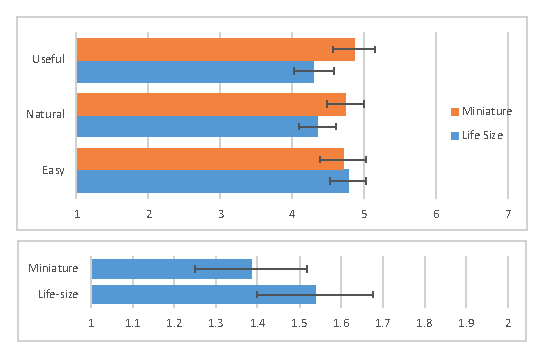
\includegraphics[width=0.8\linewidth]{images/42-placement-ismar17/images-09.eps}
    \caption{\textit{Top:} Mean values results of subjective questions grouped by condition by question. \textit{Bottom:} average ranking results of preferred condition between Life-size and Miniature; 1=most preferred, 2=least preferred. Whiskers indicate standard error.}
    \label{fig:continuum:results}
\end{figure}

Participants answered open-ended questions about the positives and negatives of each condition. Participants reported the most useful scenarios for the C1-Life-sized condition as:

\begin{itemize}
    \item \enquote{face-to-face conversations with a social contact}
    \item \enquote{when zooming into a subset group of friends}. 
\end{itemize}

Some of the positive feedback of C1-Life-sized include:

\begin{itemize}
    \item \enquote{Felt very personal, and I felt more engaged because I was actually in the situation}
    \item \enquote{Very satisfying seeing friends further out in lower fidelity. Give a real sense of good friends vs acquaintances}
\end{itemize}

While some of the negative comments on C1-Life-sized include:

\begin{itemize}
    \item \enquote{Hard to see people in the context of each other}
    \item \enquote{It was hard to get an overall perspective of all friends}
\end{itemize}
 
For the Miniature condition, participants reported this condition as useful for: 

\begin{itemize}
    \item \enquote{seeing the overall picture of social contacts} 
    \item \enquote{moving contacts between different social circles} 
\end{itemize}

Some of the positive feedback of C1-Life-sized include:

\begin{itemize}
    \item \enquote{I prefer the miniature version because I can see the whole "play space" at once}
    \item \enquote{Much better than life size to be able to see them all at once, see the big picture. Context of people relative to each other}
\end{itemize}

While others mentioned the followings as negative feedback: 

\begin{itemize}
    \item \enquote{It felt more disconnected compared to the life-size due to my position feeling further away}
    \item \enquote{Hard to select characters. Difficult to see [who is who]}
\end{itemize}

\subsection{Discussion}
% It would be good to include more discussion about the results from this user test

% Mark: It would be good to include more discussion about the results from this pilot test

% gogo: I agree. This section seems very short compared to the previous one. Also, what is the takeaway message from this section? As far as I can tell, the user preferred the miniature one, if any. Is that the one you decided to explore further? If not, why not?

% Tobias: I am missing the discussion of the insights and the directions for future work. In particular, I am missing discussions on relevance. All this should come after the results. Normally, a longer paper/thesis would have a results section which focuses on the statistical analysis but not discussion/interpretation. This is usually followed up with a discussion section which expands then on the results by offering a discussion and interpretation of these results. What do these results mean? What is the practical meaning and relevance? This section and this detailed interpretation are missing even though it is the most important. Similarly, the relevance for future work and the field of AR is missing.

The Likert scale results did not show any significant results between C1-Life-sized and C2-Miniature representation of avatars in terms of usefulness, natural or easy interactions. This indicates that both representations are valid options and depending on the use-case scenario, viewers could either see their social contacts in C1-Life-sized or C2-Miniature. There are both advantages and disadvantages for each condition drawn from the positive and negative feedback by participants. The semi-structured interview highlighted some of the positive and negative sides of each condition. This indicates that it might be ideal if the system allows for easy switching between Life-sized and Miniature placement based on the required scenarios. 


\subsection{Conclusion}

This section investigated different options of placing the social contacts; either as Life-sized avatars or as Miniature avatars. Results (Figure \ref{fig:continuum:results}) showed that participants did not have any preference between the life-size condition and the Miniature condition, and it is a matter of user preference. Therefore, in the next chapters, we focus on displaying social contact as Life-Sized.

